\chapter{绪论}

\section{乙型肝炎病毒感染、生命周期与抗病毒治疗需求}

乙型肝炎病毒（hepatitis B virus, HBV）感染是全球范围内最重要的慢性病毒感染之一，也是肝硬化和肝细胞癌（hepatocellular carcinoma, HCC）的主要病因之一。HBV感染既可表现为急性自限性肝炎，也可发展为长期持续的慢性感染；后者在长期炎症、肝细胞损伤与再生、病毒蛋白表达及宿主免疫压力共同作用下，可显著增加终末期肝病和肝癌风险\cite{dusheiko2023new,lin2020association}。虽然预防性疫苗已经显著降低了新发感染率，核苷（酸）类似物和干扰素治疗也能够有效抑制病毒复制，但现有治疗通常难以彻底清除感染细胞内的共价闭合环状DNA（cccDNA）及相关病毒遗传物质。因此，慢性HBV感染仍常需要长期治疗和随访，停药后病毒学反弹、药物耐受性以及残余肝癌风险等问题依然存在。

从药物开发角度看，HBV生命周期中的多个步骤均可能成为抗病毒干预靶点。传统核苷（酸）类似物主要抑制病毒聚合酶介导的逆转录过程，而近年来针对病毒进入、衣壳组装、cccDNA维持、病毒RNA稳定性以及宿主免疫调节等环节的策略也受到关注\cite{selzer2015assembly,taverniti2022capsid}。其中，感染性病毒颗粒的形成依赖于病毒核衣壳与包膜蛋白之间的特异性识别和装配。该过程位于病毒复制后期，直接决定成熟核衣壳能否被包膜包裹并分泌为具有感染性的Dane颗粒。若能够选择性阻断核衣壳包膜化，理论上可在不完全依赖聚合酶抑制的情况下减少感染性病毒颗粒释放，从而为开发新型抗HBV药物提供补充方向。

在这一背景下，理解HBV感染性颗粒形成的分子机制，对于寻找区别于传统聚合酶抑制的新型干预策略具有重要意义。HBV是一种有包膜的小型DNA病毒，病毒颗粒内部为由核心蛋白（hepatitis B core protein, HBc）组装而成的二十面体核衣壳，外部包裹含有乙肝表面抗原（hepatitis B surface antigen, HBsAg）的脂质膜\cite{venkatakrishnan2016structural}。HBc蛋白可通过二聚体作为基本单元自发组装成T=3或T=4对称性的核衣壳，其中T=4颗粒在体外和病毒颗粒中均较为常见。核衣壳不仅为前基因组RNA（pgRNA）和病毒聚合酶提供封装空间，也为逆转录反应提供受限的内部环境。随着pgRNA逆转录为松弛环状DNA，核衣壳逐渐成熟，并获得参与后续包膜化和分泌的能力。

HBV感染性颗粒的形成并不是核衣壳随机被细胞膜包裹的过程，而是一个需要病毒蛋白之间精确匹配的形态发生事件。成熟核衣壳需在内质网及其相关膜系统附近与HBsAg发生相互作用，随后通过细胞分泌途径释放\cite{bruss2007morphogenesis,selzer2015assembly}。这一过程具有高度选择性：一方面，未成熟核衣壳一般不能高效进入分泌途径；另一方面，HBsAg本身可以大量形成不含核衣壳的亚病毒颗粒（subviral particles, SVPs），说明表面蛋白外排与感染性病毒颗粒包膜化虽然共享部分膜运输路径，却并非完全相同的机制。因而，核衣壳与包膜蛋白之间的特异性相互作用被认为是HBV形态发生的核心调控节点。

\section{HBsAg preS区域在核衣壳包膜化中的功能}

HBsAg由同一开放阅读框通过不同翻译起始位点产生三种相关蛋白：小表面蛋白S-HBsAg、中表面蛋白M-HBsAg和大表面蛋白L-HBsAg\cite{seitz2020envelope}。三者共享S结构域；M-HBsAg在N端额外含有preS2区域；L-HBsAg进一步包含preS1和preS2区域，二者合称preS区域。遗传学研究显示，L-HBsAg和S-HBsAg对于感染性病毒颗粒的形成不可或缺，而M-HBsAg在许多实验体系中并非病毒颗粒分泌的必需组分\cite{bruss1991role,ni2010pres2}。这一现象提示，L-HBsAg特有的preS区域在病毒颗粒成熟过程中承担了特殊功能。

L-HBsAg的一个重要特征是preS区域具有双重跨膜拓扑。部分preS位于病毒颗粒外侧，能够在感染早期介导病毒与肝细胞受体NTCP结合，并参与后续入侵过程\cite{yan2012ntcp,asami2024structural}；另一部分preS则朝向病毒颗粒内侧或细胞质侧，被认为参与核衣壳包膜化。强制改变L-HBsAg拓扑、使preS仅呈外向型分布，会阻断病毒颗粒分泌而不明显影响核衣壳装配，说明内向型preS与核衣壳的接触是病毒形态发生所需的独立步骤\cite{bruss1995functions,seitz2020envelope}。因此，preS区域同时连接了HBV入侵和组装两个关键阶段，是病毒生命周期中的多功能调控区。

preS区域还具有重要的临床和病理学意义。慢性HBV感染患者中可出现自然发生的preS缺失或突变，这些变异与表面蛋白滞留、内质网应激、免疫逃逸、病毒颗粒分泌异常以及HCC发生风险升高有关\cite{lin2020association,peiffer2018divergent}。从机制角度看，preS突变不仅可能影响受体结合和抗原性，也可能改变L-HBsAg与核衣壳的相互作用，进而影响病毒颗粒形成效率和病毒群体组成。因此，解析preS如何识别HBc，不仅有助于理解HBV形态发生，也有助于解释慢性感染过程中某些preS变异被选择和维持的原因。

围绕preS功能的早期遗传学和生化研究已经证明，L-HBsAg的preS区域与HBc核衣壳之间存在功能性联系。preS1内部的一段短线性序列被证实对病毒颗粒形成至关重要，相关区域的缺失或突变会显著损害Dane颗粒分泌，但未必影响表面蛋白形成亚病毒颗粒\cite{bruss1995functions,bruss1997short}。Bruss进一步通过linker substitution和双丙氨酸扫描突变，将这一功能区缩小到preS1 C端约27个氨基酸范围内；这些突变体仍可产生相对稳定的L蛋白并与S蛋白共同形成亚病毒颗粒，但部分突变显著削弱感染性病毒颗粒释放\cite{bruss1997short}。根据该研究对preS功能区的定位，preS 87--114可被视为preS与core发生关键相互作用并支持包膜化的核心区域，而不是单纯影响表面蛋白表达或分泌的区域。

\begin{figure}[htbp]
  \centering
  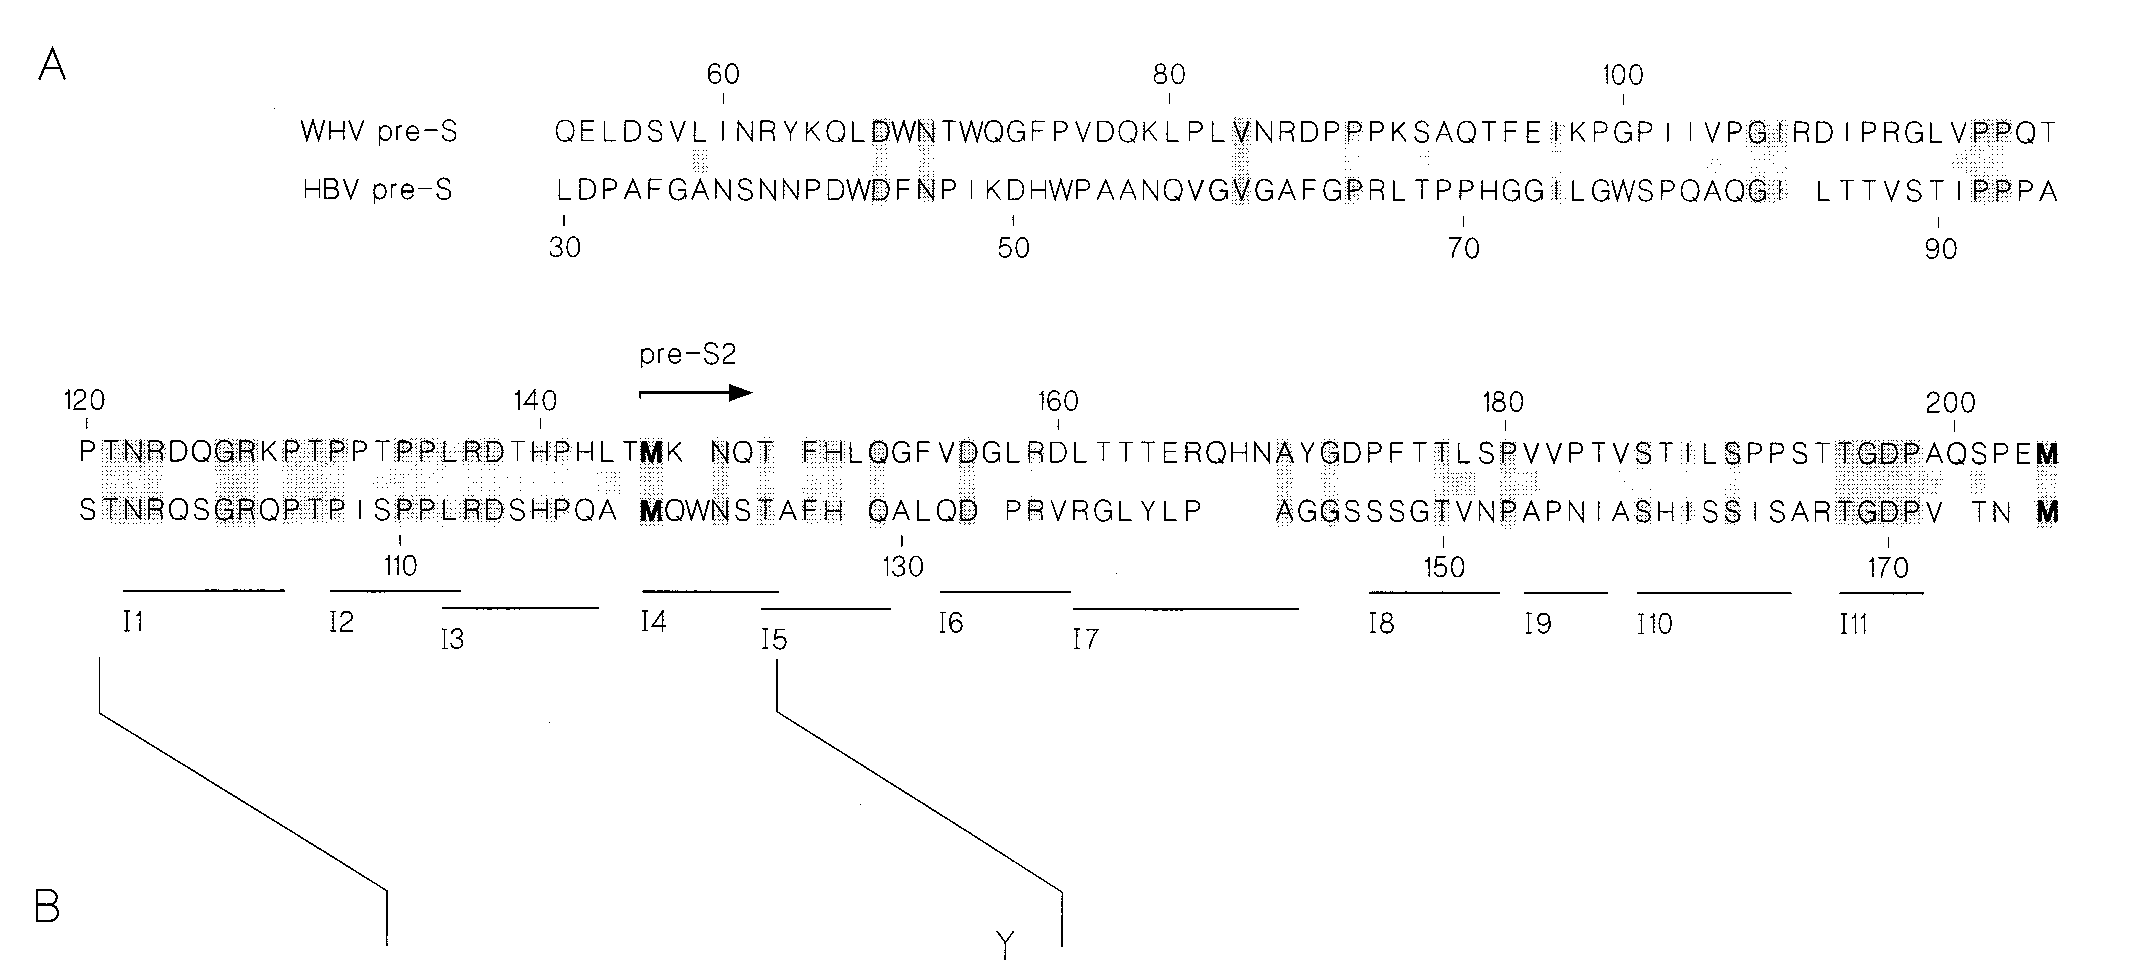
\includegraphics[width=0.86\textwidth]{figures/introduction/bruss1997_pres_mutant_map.png}
  \par\medskip
  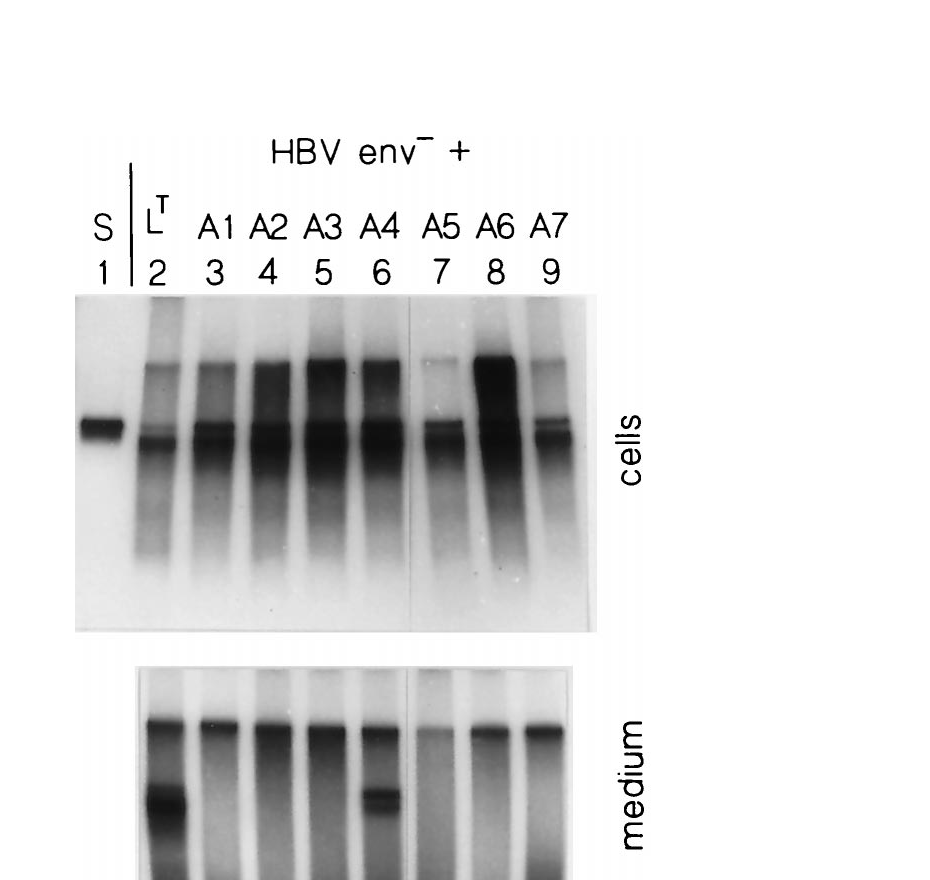
\includegraphics[width=0.42\textwidth]{figures/introduction/bruss1997_virion_complementation.png}
  \caption{preS短线性功能区的早期定位。上图显示Bruss构建的preS突变定位图；下图显示部分双丙氨酸突变体在L蛋白阴性HBV基因组互补实验中的病毒颗粒释放表型。该区域的突变可在保留表面蛋白相关分泌能力的同时削弱病毒颗粒形成，提示其可能参与核衣壳识别和包膜化过程。图片截取自Bruss的研究\cite{bruss1997short}。}
  \label{fig:bruss1997-pres-core-region}
\end{figure}

除preS区域外，S结构域胞质环也被报道具有核心颗粒结合能力。Poisson等利用体外多肽和核心颗粒结合实验发现，preS1相关片段和S区胞质环均可与HBc颗粒发生相互作用\cite{poisson1997both}。后续研究通过ELISA、BIAcore和合成多肽进一步支持了HBV包膜化过程中存在多点接触的模型，认为preS与S区胞质环可能共同稳定核衣壳--包膜复合物\cite{choi2004quantitative,muhamad2015peptide}。然而，这些实验多数依赖短肽、固定化蛋白或体外重构体系，难以完全反映膜环境中全长表面蛋白和核衣壳之间的动态接触。

细胞水平研究也支持L-HBsAg在介导核衣壳--包膜相互作用中的关键作用。共表达实验显示，L-HBsAg能够促进核心蛋白向核周或膜相关区域重新定位，并与核心蛋白发生可检测的共沉淀；相较之下，单独S-HBsAg与核心蛋白之间的相互作用较弱\cite{pastor2019direct}。此外，preS1--preS2衔接区的缺失可破坏核心蛋白重定位和共沉淀，提示该区域对于形成有效的核心蛋白--包膜蛋白复合物十分关键。这些发现将早期多肽研究与细胞内形态发生过程联系起来，进一步强调preS区域是HBV包膜化研究的中心对象。

\section{HBc--preS结合区域与药物靶向潜力}

尽管HBc--preS相互作用已被多种实验证据支持，其高分辨率结构基础长期缺乏。造成这一困难的原因之一在于，单个preS片段与核衣壳的相互作用可能较弱，而真实病毒颗粒中L-HBsAg和HBc二聚体均以多拷贝形式存在，多价效应可能显著增强整体结合稳定性。基于Bruss对preS短线性功能区的定位，preS 87--114被认为是连接L-HBsAg和core的关键区域\cite{bruss1997short}。因此，围绕该区域建立非感染性体外互作检测体系，有助于在较高生物安全性和可控性条件下解析HBc--preS相互作用。

从药物靶向角度看，HBc表面的可结合口袋为干预核衣壳--包膜蛋白相互作用提供了潜在切入点。Makbul等在HBc衣壳样颗粒中观察到Triton X-100（TX100）可结合核心蛋白二聚体界面附近的疏水口袋，ITC测得其与HBc颗粒的结合处于微摩尔量级，并且冷冻电镜密度显示TX100位于由HBc链间残基围成的特定口袋内\cite{makbul2021binding}。该研究说明，HBc表面除经典CAM口袋外还存在能够容纳疏水小分子的局部结构，为后续评价小分子是否影响HBc--preS结合提供了结构线索。

\begin{figure}[htbp]
  \centering
  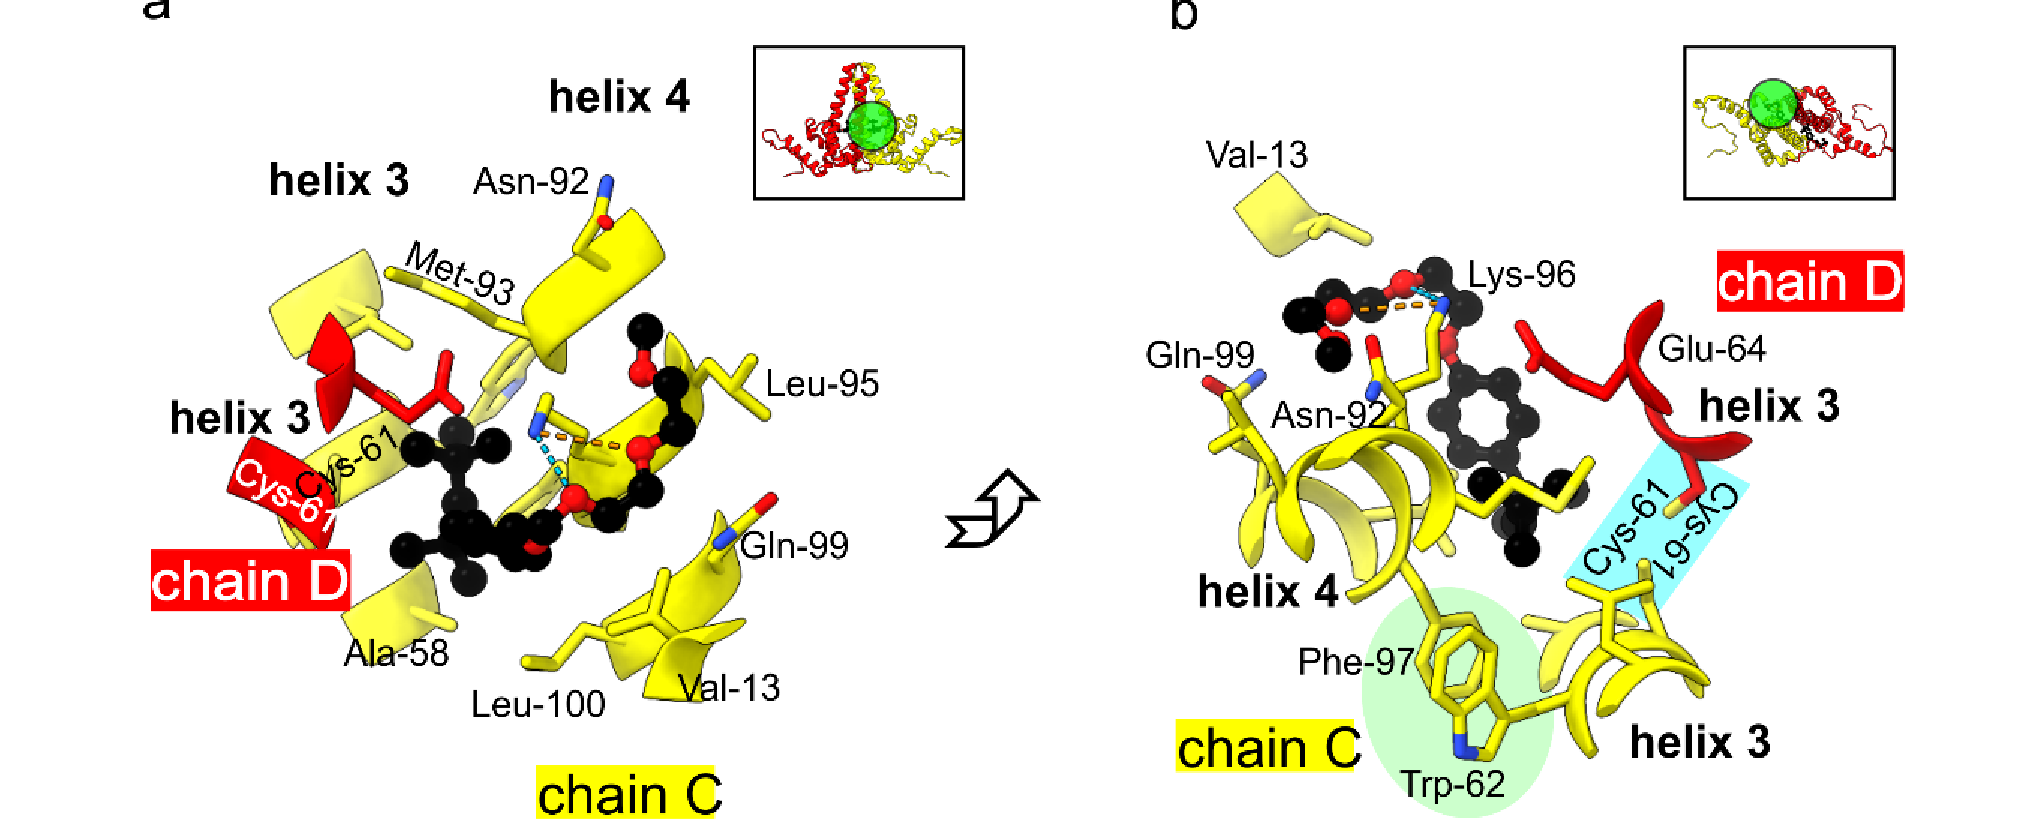
\includegraphics[width=0.70\textwidth]{figures/introduction/makbul2021_tx100_hbc_pocket.png}
  \caption{Triton X-100结合HBc二聚体疏水口袋的结构示意。TX100位于HBc链C和链D形成的二聚体界面附近，并被特定疏水口袋容纳。图片截取自Makbul等的研究\cite{makbul2021binding}。}
  \label{fig:makbul2021-tx100-pocket}
\end{figure}

香叶醇（geraniol）也被报道能够直接结合HBc核心蛋白。Khayenko等结合ITC和冷冻电镜发现，geraniol以微摩尔亲和力结合HBc中心疏水口袋，冷冻电镜图中可在不对称单位内多个疏水口袋观察到geraniol相关密度，并且其结合位置与TX100结合位点发生空间重叠\cite{khayenko2024induction}。因此，TX100和geraniol并不只是非特异性疏水添加剂，而是能够占据HBc特定疏水口袋的小分子。这些已发表研究提示，HBc疏水口袋具有被小分子结合和调控的可能性。

\begin{figure}[htbp]
  \centering
  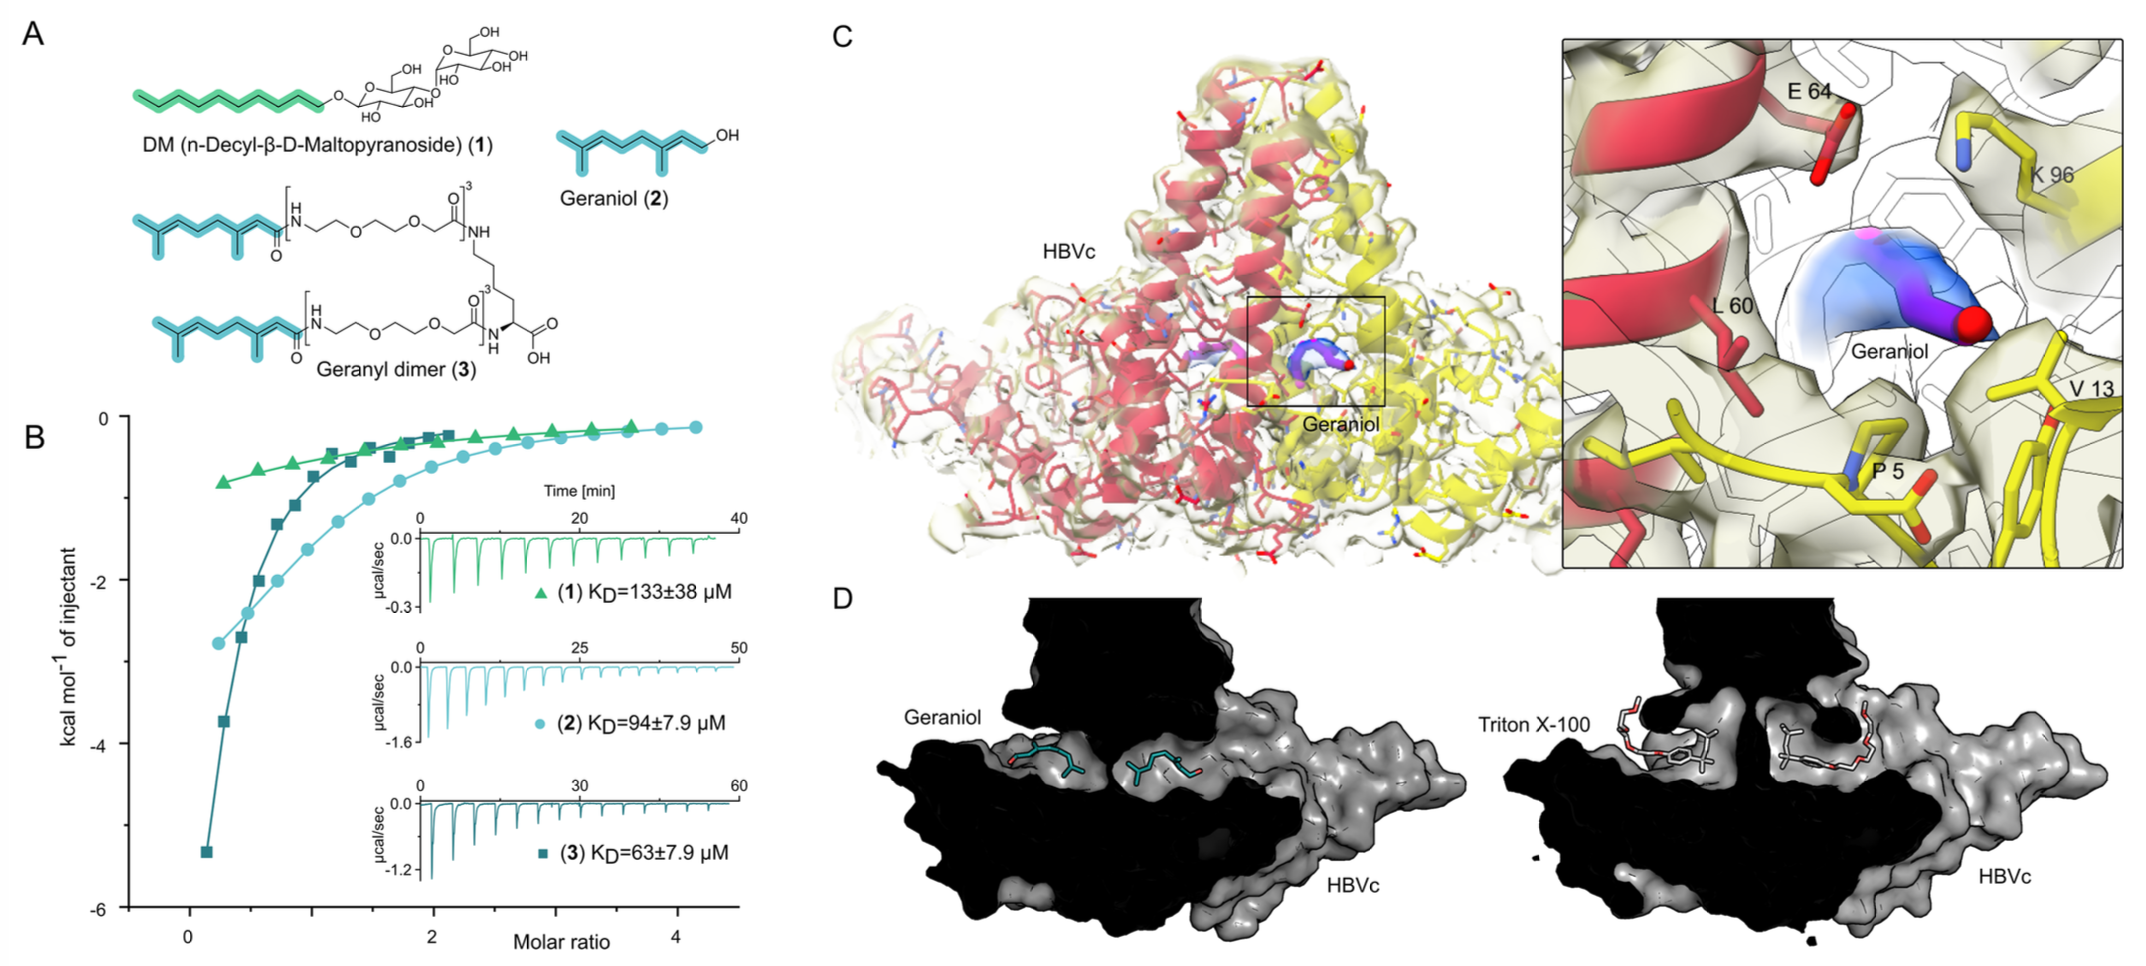
\includegraphics[width=0.82\textwidth]{figures/introduction/khayenko2024_geraniol_hbc_pocket.png}
  \caption{香叶醇（geraniol）结合HBc中心疏水口袋及其与TX100结合位点的比较。结构和热力学数据支持geraniol可与HBc核心蛋白直接相互作用，并结合在可容纳疏水分子的特定口袋中。图片截取自Khayenko等的研究\cite{khayenko2024induction}。}
  \label{fig:khayenko2024-geraniol-pocket}
\end{figure}

在上述已发表口袋结合研究的基础上，本实验室尚未发表的pull-down实验进一步检测了TX100和geraniol是否会影响preS 87--114与HBV core的体外结合。在Strep-tag pull-down实验中，研究者先将HBV core与TX100或geraniol预孵育，再加入带Strep标签的三聚化preS 87--114构建体；结果显示，在preS和输入core信号仍可检测的条件下，小分子处理组pull-down中的anti-core信号明显降低。这一结果支持TX100和geraniol在该体外体系中能够削弱preS 87--114对core的结合。由于该部分数据仍处于投稿阶段，本文仅将其作为本实验室未发表的初步机制性证据进行谨慎表述，不将其列入参考文献。

\begin{figure}[htbp]
  \centering
  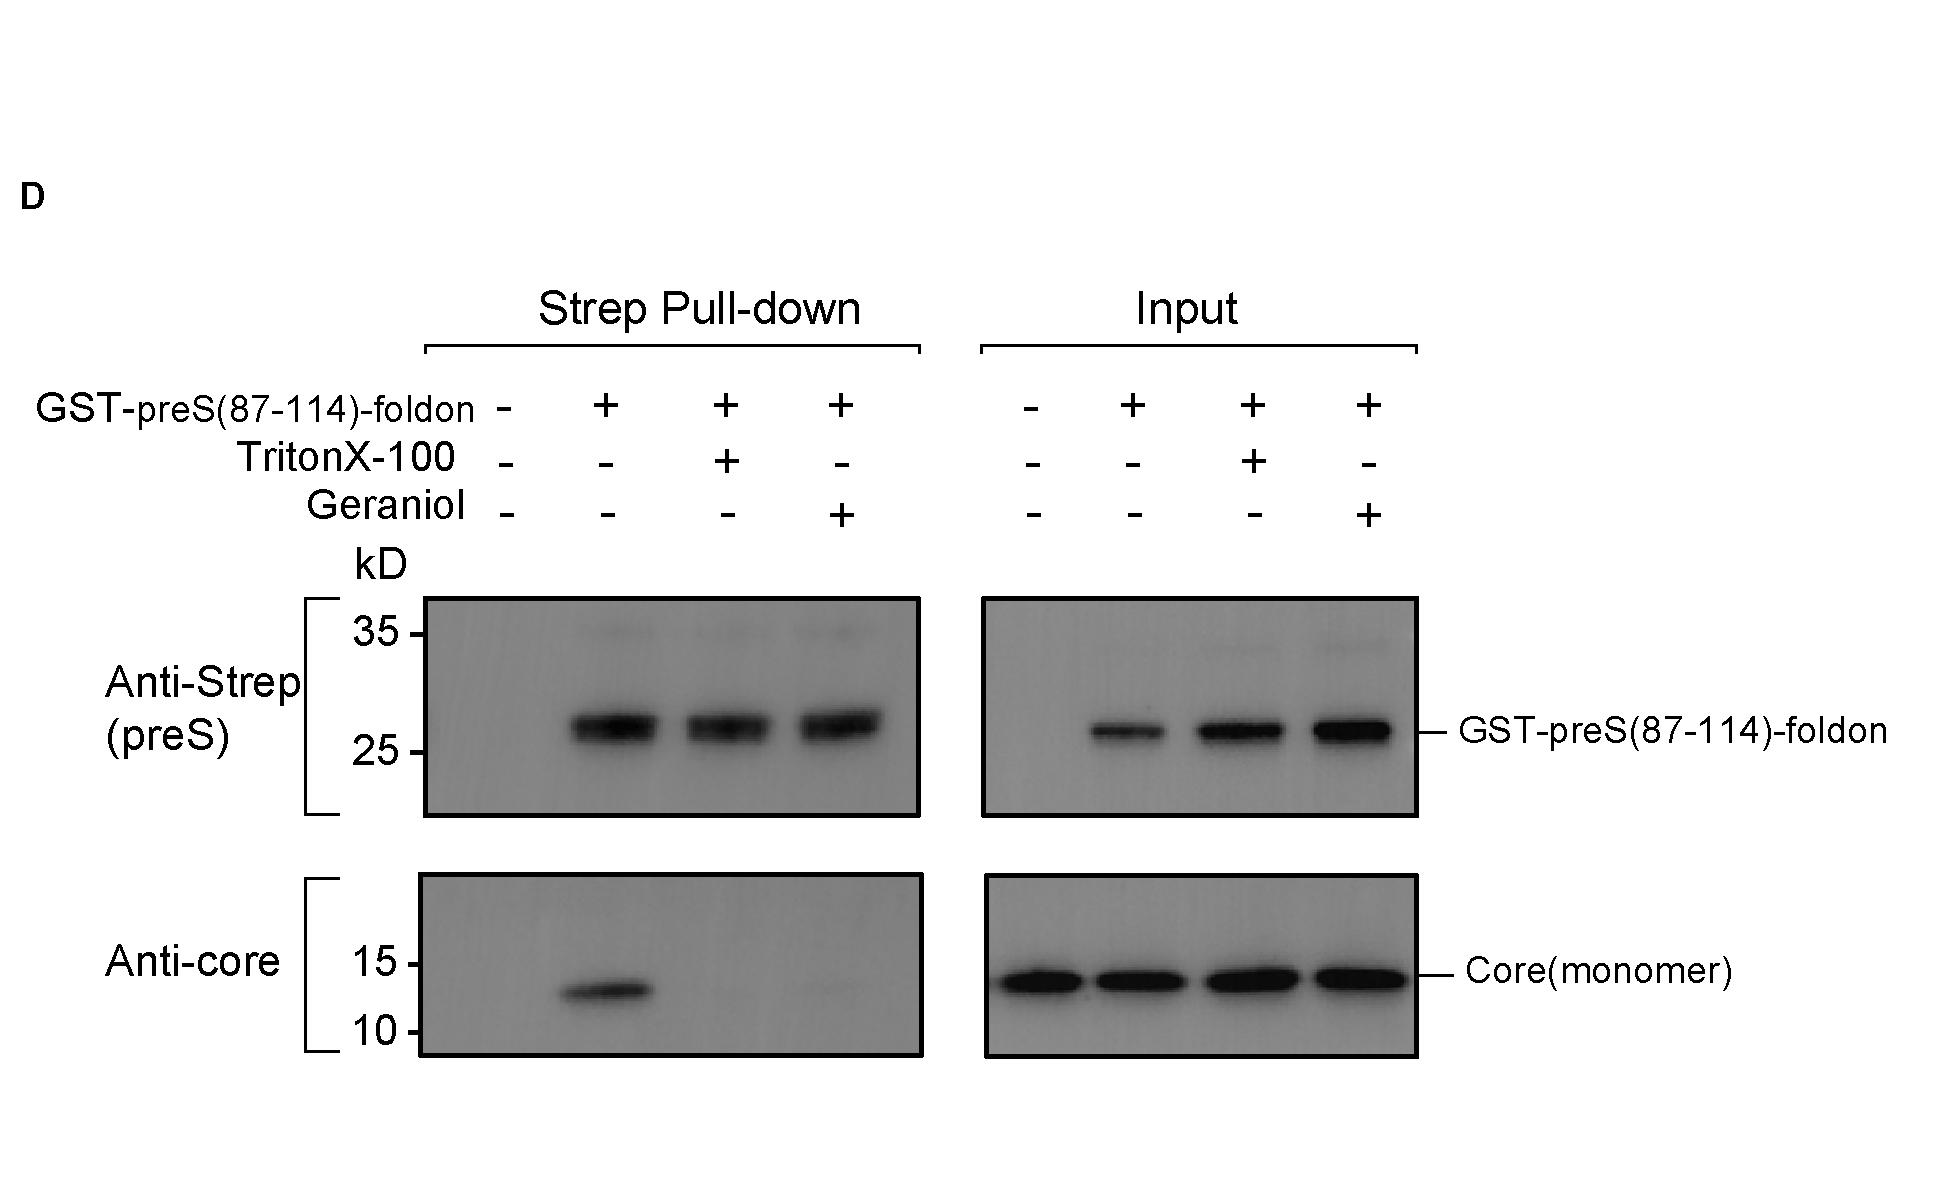
\includegraphics[width=0.68\textwidth]{figures/introduction/lab_unpublished_fig4d_pulldown_small_molecules.png}
  \caption{TX100和geraniol抑制preS 87--114--HBc体外结合的pull-down证据。Strep-tag pull-down显示，核心蛋白经TX100或geraniol预孵育后，随preS 87--114被拉下的anti-core信号降低，而输入样品中的核心蛋白和preS信号仍可检测。该图来自本实验室尚未发表的投稿中研究，因此不列入参考文献。}
  \label{fig:lab-unpublished-small-molecule-pulldown}
\end{figure}

这些发现使HBc--preS界面从单纯的病毒形态发生机制问题进一步转化为潜在药物靶点问题：若小分子能够稳定占据或调控该口袋，就可能阻断包膜化所需的关键识别步骤，从而减少感染性病毒颗粒形成。

从药物开发角度看，当前核心蛋白相关策略主要集中于衣壳组装调节剂（capsid assembly modulators, CAMs）。CAMs通过结合HBc二聚体界面附近的口袋影响核心蛋白装配、核衣壳稳定性或pgRNA封装，从而抑制病毒复制\cite{taverniti2022capsid,luo2021core}。然而，HBc不仅是衣壳组装单元，也是成熟核衣壳被包膜选择性识别的表面平台。与直接扰动衣壳组装不同，靶向HBc--preS界面有望选择性干预病毒生命周期后期的包膜化步骤，为核心蛋白靶向药物提供另一种机制类型。

既往小分子筛选研究已经证明，阻断核心蛋白与表面蛋白之间的相互作用具有可行性。Asif-Ullah等通过ELISA检测HBc与preS结合并筛选化合物，发现部分小分子能够抑制该相互作用，并降低细胞中HBV颗粒释放水平\cite{asifullah2006compounds}。虽然这些早期化合物距离临床药物仍有较大距离，但它们从概念上证明了核衣壳--包膜蛋白界面具有可干预性。TX100和geraniol的HBc口袋结合研究则进一步提示，后续药物设计可以围绕HBc表面可成药口袋、竞争机制和体外互作验证进行理性优化。

从生物安全和实验可控性角度看，利用非感染性重组蛋白、合成片段或报告系统研究HBc--preS结合，是解析该界面和评估候选抑制物的合适路径。此类体系不涉及感染性病毒扩增或病毒传播能力增强，而是将问题聚焦于纯化组分之间的物理相互作用及其抑制规律。对于毕业论文研究而言，建立稳健的体外定量平台，比较preS 87--114相关构建体和小分子竞争效应，既能够服务于基础机制研究，也能够为后续更严格的药物筛选和细胞水平验证提供前期依据。

\section{本研究的目的与意义}

综上所述，HBc--preS相互作用是HBV感染性颗粒形成中的关键步骤，也是连接结构生物学机制研究与新型抗病毒药物开发的重要界面。已有遗传学、生化和细胞实验表明preS区域参与核衣壳包膜化；Bruss的功能定位研究进一步支持preS 87--114是与core发生关键相互作用的区域\cite{bruss1997short}。同时，TX100和geraniol等小分子能够结合HBc特定疏水口袋，为探索小分子干预HBc--preS相互作用提供了依据。该方向仍需要更多定量实验支持，特别是在不同preS构建体和不同小分子浓度条件下，对HBc--preS结合强弱进行系统比较。

本研究旨在建立并应用基于NanoBiT的HBc--preS体外定量检测平台，在安全、可控的非感染性重组蛋白体系中验证HBV核衣壳与HBsAg preS区域的相互作用。研究重点包括：比较野生型与突变preS片段的HBc结合能力；评估Triton X-100、geraniol等小分子对HBc--preS相互作用的抑制效果；并结合已发表口袋结合研究和本研究体外实验结果解释小分子竞争所反映的界面机制。通过这些工作，可以进一步验证preS 87--114与HBc相互作用在HBV包膜化中的功能意义，为靶向核衣壳--包膜蛋白相互作用的新型抗病毒策略提供实验依据。
